 	
\documentclass[a4paper,12pt, titlepage]{report}

\usepackage[a4paper, margin=0.75in]{geometry}
\usepackage{graphicx}
\usepackage{listings}
\usepackage{xcolor}
\usepackage[hyphens]{url}
\usepackage{hyperref}
\usepackage[export]{adjustbox}
\usepackage{subfig}
\usepackage{pdfpages}




\definecolor{mGreen}{rgb}{0,0.6,0}
\definecolor{mGray}{rgb}{0.5,0.5,0.5}
\definecolor{mPurple}{rgb}{0.58,0,0.82}
\definecolor{backgroundColour}{rgb}{0.95,0.95,0.92}

\lstdefinestyle{CStyle}{
    backgroundcolor=\color{backgroundColour},   
    commentstyle=\color{mGreen},
    keywordstyle=\color{magenta},
    numberstyle=\tiny\color{mGray},
    stringstyle=\color{mPurple},
    basicstyle=\footnotesize,
    breakatwhitespace=false,         
    breaklines=true,                 
    captionpos=b,                    
    keepspaces=true,                 
    numbers=left,                    
    numbersep=5pt,                  
    showspaces=false,                
    showstringspaces=false,
    showtabs=false,                  
    tabsize=2,
    language=C
}

\lstset{escapechar=@,style=CStyle}




\begin{document}

\begin{titlepage} % Suppresses headers and footers on the title page

	\centering % Centre everything on the title page
	
	\scshape % Use small caps for all text on the title page
	
	
	\includegraphics[scale=0.2,right]{"assets/UoN eee".png}
	
	%------------------------------------------------
	%	Title
	%------------------------------------------------
	 
	\rule{\textwidth}{2pt}\vspace*{-\baselineskip}\vspace*{2pt} % Thick horizontal rule
	
	\vspace{0.75\baselineskip} % Whitespace above the title
	
	{\LARGE Applied EEE Construction Project:\\ Lab Report 2: \\ \ Subsystem design and Main vehicle integration\\} % Title
	
	\vspace{0.75\baselineskip} % Whitespace below the title
	
	\rule{\textwidth}{2pt} % Thick horizontal rule
	
	\vspace{2\baselineskip} % Whitespace after the title block
	
	%------------------------------------------------
	%	Subtitle
	%------------------------------------------------
	
	Lab report from sessions 3 \& 4 of the applied EEE construction Project % Subtitle or further description
	
	\vspace*{3\baselineskip} % Whitespace under the subtitle
	
	%------------------------------------------------
	%	Editor(s)
	%------------------------------------------------
	

	
	\vspace{0.5\baselineskip} % Whitespace before the editors
	
	{\scshape\Large Michael Bagge-Hansen } % Editor list

	\href{mailto:eeymb8@Nottingham.ac.uk}{eeymb8@Nottingham.ac.uk}
	
	\vspace{1\baselineskip}
	
	Abstract: \\
	\textit{
	This report outlines the plan, testing and build of the autonomous parking subsystem. The system utilises ultrasonic sensors mounted to servos, to map out the parking space. to improve accuracy the servos only move to 3 set positions. due to a deficit of pins the serial monitor was out of service, this made debugging the system very difficult, and as a result did not meet the brief within the give time.    
	}	
	
	\vfill % Whitespace between editor names and publisher logo

	
	
	%------------------------------------------------
	%	Publisher
	%------------------------------------------------
	
%	\plogo % Publisher logo
	
	\vspace{0.3\baselineskip} % Whitespace under the publisher logo
	
	November 2019 % Publication date
	
	{\large The University of Nottingham} % Publisher

\end{titlepage}

\setcounter{page}{0}

\tableofcontents

		\chapter{Introduction}
		
This report summarises the objectives achieved in sessions 5 \& 6 of the construction project. The main goal of which was to use a raspberry pi with open CV to create computer vision systems such as line following and symbol detection. The aim for the sessions is to complete a series of challanges around a track shown in figure \ref{fig:track}. 

\begin{figure}[h]%track
	\centering
	\includegraphics[width = 0.5\textwidth]{"assets/track"}
	\caption{consept drawing for track}
	\label{fig:track}
\end{figure}

		
	\section{Raspberry pi}
The raspberry pi is a small single-board computer designed for projects such as this. It has a quad core 1.2 GHz ARM processor \cite{pi_product_page}, a good choice for our project as it is powerful enough to run most programs with ease and are cheap enough to keep the price of the product to £32 \cite{pi_product_price}. The Raspberry pi has easy access to GPIO pins allowing for communication to the arduino's. The Pi's included ports; HDMI, micro USB for power, Ethernet and 4 USB 2 ports, allow for easy setup, shown in section \ref{sec:pi_setup}.\\ The pi runs Raspbian, based on Debian, a linux os. Raspbian is basic, build for beginners. It launches to a desktop environment that is lightweight, perfect for running on the ARM possessor. It comes with the apt repository allowing for easy install of many applications. \\
The pi is an excellent choice for this project due to its from factor, price, easy setup and its large community, due to its popularity there is a wide range of support and documentation, meaning the problems you might have will already have been solved by someone else.    
	\section{Open CV}
	
Open CV is a c++ and python library for Computer vision. It has many advanced features such as object detection and 3D transformation, however for this project we will only be using the more basic functions as follows: masking - creating a black and white image with white being only a specified color range and black being every other color. Create contour \& poly contour - create an line at all the edges between the black and white, simplify the contour to a few straight lines.\\
To get used to the library a task was assigned who's objective was to find the main color in a image, completed in appendix \ref{apx:open_cv_task}.
	
		\chapter{Physical Systems}
	\section{Audio Amplifier}

In order to increase the outputs available from the car	an Set of speaker was to be added. This is to be made with an LM3886 op amp and will use the Raspberry pi's audio jack and be powered from the 5v and ground GPIO pins on the pi. Using the GPIO pins on the raspberry pi as sound output was another option, 2 variations on this where explored. to have make an i2c sound card or to connect the amplifier to the PWM GPIO pins.

\paragraph*{PWM pins}
As shown in figure \ref{fig:pi_audio_schematic}, the headphone jack is connected to PWM pins: PWM1 to left channel, PWM0 to the right. To access these channels with the GPIO pins 12 and 13 on ALT 0 \cite{GPIO_functions}.\\
this would allow for the circuit to improve the sound quality and would make the design of the vehicle more streamlined. This would be a good option if there was more of a space concern and would be ideal if custom PCBs could be made as there would be no bulky connector between the pi and the amplifier, however as all the components are made by hand it is easier to make everything on strip-board meaning the circuit would be much larger than necessary. 

\begin{figure}[h]%headphone jack circuit
	\centering
	\includegraphics[width = 0.8\textwidth]{"assets/pi_audio_schematic"}
	\caption{Raspberry pi headphone jack circuit \cite{ras_pi_schematic}} 
	\label{fig:pi_audio_schematic}
\end{figure}

\paragraph*{i2c soundcard}
An i2c sound card would have similar benefits to the PWM pin option. It would also have the benefits of allowing audio input, which the raspberry pi does not have out of the box and would allow other devises on the bus to communicate. However it would also have similar downsides to the PWM pins as it would require a complex circuit with specialised chipsets as well, thereby not making it a viable option.  

\paragraph*{Headphone jack}
This system allows the circuit to be more plug and play, allowing for easy installation and debugging as the points of failure are easy to test individually. the circuit would be fairly simple as it would not require any other processing other than the amplifier its self. This is the most viable option considering the  of the vehicle, so it was chosen as the continued design.

\subsection{Circuit}

\begin{figure}[h]%audio amp circuit	
	\centering
	\includegraphics[width = 0.6\textwidth]{"assets/audio_amplifier"}
	\caption{Audio amplifier circuit \cite{amp_circuit}}
	\label{fig:amp_circuit}
\end{figure}

This amplifier circuit shown in figure \ref{fig:amp_circuit} is from a website shown in \cite{amp_circuit}, it is matched with $8 \Omega, \, 0.08W$ speakers from RS Components \cite{speakers} they can be mounted to a pcb and are low resistance enough to be powered of the 5v supply from the GPIO pins on the raspberry pi. 2 of these circuits are constructed on a single pcb to keep the vehicle compact. The circuit's power is connected to a 2 pin header on the +5v and ground on the Raspberry pi Breakout Board though a screw terminal block, this allows the wires to be shortened or lengthened to suit the layout of the vehicle. The input signal is also connected by screw terminal blocks, and connected to the audio jack on the raspberry pi. Assembly of the audio amplifier shown in figure \ref{fig:amplifyer_pcb}. 

\begin{figure}[h]%amp accembley
    \centering
    \subfloat[Amplifier PCB front]{{\includegraphics[width=7cm]{"assets/amp_front"} }}%
    \qquad
    \subfloat[Amplifier PCB back]{{\includegraphics[width=7cm]{"assets/amp_back"} }}%
    \caption{Amplifier PCB}%
    \label{fig:amplifyer_pcb}%
\end{figure}

	\section{I2C level shifter}
	
The I2C bus on the arduino runs off 5v, whereas the I2C bus on the raspberry pi runs off 3.3v. Supplying the raspberry pi's I2C pins with 5v could damage the components of the pi, potentially making it unusable. Similarly with the arduino being fed 3.3v, although it would be able to handle the voltage it will behave unpredictably making it unusable as a communication signal.\\ \\
To fix this a level shifter is to be designed, this will allow the 3.3v signal from the Pi to be pulled up to 5v to allow the arduino to read it, and drop the 5v signal to 3.3v to prevent damage to the raspberry pi. Circuit diagram in figure \ref{fig:i2c_level_shifter_diagram}

\begin{figure}[h]%i2c level shifter diagram
	\centering
	\includegraphics[width = 0.6\textwidth]{"assets/i2c_shifter_diagram"}
	\caption{i2c level shifter circuit diagram \cite{level_shifter}}
	\label{fig:i2c_level_shifter_diagram}
\end{figure}

	\section{Sensors with Arduino}
	
As part of the specification it was required that the vehicle had some ultrasonic sensors, as well as this the camera was to have pitch control with a servo. It was decided that these sensors and the servos would be controlled with a arduino nano and communicate with the raspberry pi over i2c. This was decided to do this instead of connecting directly to the raspberry pi because the raspberry pi does not have libraries to control servos and ultrasonic sensors meaning custom code would have to be written whereas not much would be needed for the arduino. This approach would also leave room for expansion, for example on the circuit board there are pin headers for a RF module, allowing for the car to be remove controlled. Circuit assembly shown in figure \ref{fig:sensor_circuit}. Code for system shown in   
	
\begin{figure}[h]%sensors circut
    \centering
    \subfloat[Sensor circuit front]{{\includegraphics[width=7cm]{"assets/sensor_front"} }}%
    \qquad
    \subfloat[Sensor circuit back]{{\includegraphics[width=7cm]{"assets/sensor_back"} }}%
    \caption{Sensor circuit}%
    \label{fig:sensor_circuit}%
\end{figure}


	\section{Raspberry Pi \& Camera}
\subsection{setup}
\label{sec:pi_setup}
The setup for the raspberry pi is fairly simple, everything needed is on the os install, only thing needed to adjust is the password to prevent unauthorised use with the command \texttt{passwd pi}. Also to allow open cv programs with windows to run from an ssh terminal X11 forwarding should be enabled in the ssh config file: \texttt{$ /ect/ssh/ssh\_config $}. 
\\ 
the only issue is connecting to Eduroam as the network is not supported by the built in systems on Raspbian. to access the network the instructions in appendix \ref{apx:wifi_instructions}


The camera is a camera sold and manufactured by the raspberry pi foundation, it uses a Sony IMX219 8-megapixel sensor\cite{pi_cam_product}, found in figure \ref{fig:pi_camera}.\\
To test the camera the \texttt{raspistill} is used, buy typing \texttt{raspistill -o imgage.jpg} an image file of the camera feed will be generated. Systems build into Linux will allow openCV to interface with the camera seamlessly

\begin{figure}[h]%i2c level shifter diagram
	\centering
	\includegraphics[width = 0.5\textwidth]{"assets/pi_camera"}
	\caption{pi camera\cite{pi_cam_product} }
	\label{fig:pi_camera}
\end{figure}

\subsection{i2c communication}
To communicate with the arduinos on the vehicle the library Pi2c, from Johnny Sheppard on GitHub \cite{pi2c}. The functions from the library are shown in listing \ref{lst:pi2c_commands}

\begin{lstlisting}[language=c,caption={i2c commands example file \cite{pi2c}},label={lst:pi2c_commands}]
#include "pi2c.h"
int main(){
    Pi2c arduino(7); //Create a new object "arduino" using address "0x07"
    char receive[16]; //Create a buffer of char (single bytes) for the data

    //Receive from the Arduino and put the contents into the "receive" char array
    arduino.i2cRead(receive,16);
    //Print out what the Arduino is sending...
    std::cout << "Arduino Says: " << receive << std::endl;

    //Send an 16 bit integer
    arduino.i2cWriteArduinoInt(4356);

    return 0;
}
\end{lstlisting}

\label{sec:i2c_on_pi}
	
	\section{Motor Control}
	
The motors on the vehicle are powered by H-bridge circuits, they connect the 15v battery voltage to the motor through 2 of 4 MOSFETS, depending on the pair that is activated the current will flow in either direction across the motor making bi-directional control available, shown in figure \ref{fig:h-bridge_diagram}.  
\begin{figure}[h]%h-bridge diagram
    \centering
    \subfloat[motor direction 1]{{\includegraphics[width=5cm]{"assets/h-bridge_a"} }}%
    \qquad
    \subfloat[motor direction 2]{{\includegraphics[width=5cm]{"assets/h-bridge_b"} }}%
    \caption{H-bridge operation \cite{h-bridge}}%
    \label{fig:h-bridge_diagram}%
\end{figure}

2 of the MOSFETS are PWM, allowing for speed control of the motors. PWM or pulse width modulation is a way of varying the power of a input signal, it will rapidly switch on and off the signal in pulses, and adjusting the width of there pluses to change the power of the signal.\\
The cars motors are controlled with an arduino, so to control the motors from the raspberry pi communication code must be written.

\begin{figure}[h]%V1 control code flowchart
	\centering
	\includegraphics[width = 1\textwidth]{"assets/control_V1_flowchart"}
	\caption{motor control code V1 flowchart}
	\label{fig:control_V1_flowchart}
\end{figure}

		\chapter{Line Following System}
		
	\section{Version 1}

The design for the first version of the line following system was to split the camera feed into 3 sections, left, right and centre. Then depending which section had the most number of pixels, move the car in that direction. this was based on the infrared line following, there where 2 sensors on either side of the line would trigger a movement to either side.   

\begin{figure}[h]%V1 line following flowchart
	\centering
	\includegraphics[width = 1\textwidth]{"assets/line_following_V1_flowchart"}
	\caption{line following V1 flowchart}
	\label{fig:line_following_V1_flowchart}
\end{figure}

this version did not work as there was not enough fine adjustment to be made, this causes the vehicle to over correct often. 

	\section{Version 2}

Version 2 of the Line following system uses the open cv library more, it finds the x value of the line. With this value it will turn left for negative values, right for positive values, for a time based on the x values, the do nothing range and the scale, both of which is passed as runtime arguments to allow to for quick adjustment. 
		
\begin{figure}[h]%V2 line following flowchart
	\centering
	\includegraphics[width = 1\textwidth]{"assets/line_following_V2_flowchart"}
	\caption{line following V2 flowchart}
	\label{fig:line_following_V2_flowchart}
\end{figure}

This version also over corrected, as there is the fine control is would suggest there may be a problem where the delay between the camera feed and the motor commands or the motors are not precise enough to make fine enough adjustments. 

		\chapter{Symbol Detector Systems}
Among the systems required for the vehicle is a symbol detection system, this is necessary to include this system as it will control the triggering of the other systems on the car. For example, if the shape counting system was running constantly it would count shapes from random parts of the camera feed, thereby causing an inaccurate reading. A trigger for theses systems also decreases the load on the raspberry pi, this will allow for more complicated systems to be running constantly as there would be more free processing power.\\ \\
For the track shown in [intro figure] there are a few symbols that are required to be detected, examples of which are shown in figure \ref{fig:symbol_example}.

\begin{figure}[h]%symbols
    \centering
    \subfloat[Blue shortcut]{{\includegraphics[width=5cm]{"assets/symbols/BlueShortCut"} }}%
    \qquad
    \subfloat[Shape counter]{{\includegraphics[width=5cm]{"assets/symbols/ShapeCounter"} }}%
    \caption{Examples of symbols}%
    \label{fig:symbol_example}%
\end{figure}

The design of the Symbol detector is as follows: first a mask is created for pink pixel, contours are created of this map and then simplified. The largest rectangular contour is assumed to be the outside frame and is passed through a transform perspective function witch will convert the feed into a flat image the same size as the symbol files. then the system loops through all the symbols, and compares black and white versions of the symbols to the image, the most like symbol will be outputted.     

\begin{figure}[h]%symbol detection flowchart
	\centering
	\includegraphics[width = 1\textwidth]{"assets/symbol_detect_flowchart"}
	\caption{flowchart}
	\label{fig:symbol_detect_flowchart}
\end{figure}


\begin{figure}[h]%symbol detected
    \centering
    \subfloat[No symbol detected]{{\includegraphics[width=5cm]{"assets/symbol_test_a"} }}%
    \qquad
    \subfloat[Shape counter detected]{{\includegraphics[width=5cm]{"assets/symbol_test_b"} }}%
    \qquad
    \\
    \subfloat[Blue shortcut detected]{{\includegraphics[width=5cm]{"assets/symbol_test_c"} }}%
    \qquad
    \subfloat[Stop light detected]{{\includegraphics[width=5cm]{"assets/symbol_test_d"} }}%
    \caption{Symbol detection tests}%
    \label{fig:symbol_example}%
\end{figure}

		
		\chapter{Other Systems using Open CV}
		
	\section{Stop Light Detection}
	
To create the stop light detection, first the image was cropped around the green light and the red light separately, this is done to remove background of white pixels. Then the 2 images are compared to find the most white pixels, which ever has most is the light that is on   

\begin{figure}[h]%stop light detection flowchart
	\centering
	\includegraphics[width = 1\textwidth]{"assets/stop_light_detect_flowchart"}
	\caption{flowchart}
	\label{fig:stop_light_detect_flowchart}
\end{figure}

\begin{figure}[h]%stop light detected
    \centering
    \subfloat[Green light detected]{{\includegraphics[width=5cm]{"assets/stop_light_green"} }}%
    \qquad
    \subfloat[Red light detected]{{\includegraphics[width=5cm]{"assets/stop_light_red"} }}%
    \caption{Stop light detection}%
    \label{fig:symbol_example}%
\end{figure}
	
	\section{Shape Counting}
	
To complete the shape counting system first the image was cropped around the blue border. then a mask of the shapes was made, the shapes where counted by creating contours of the mask and counting those contours. 
	
\begin{figure}[h]%shape counter flowchart
	\centering
	\includegraphics[width = 1\textwidth]{"assets/shape_counter_flowchart"}
	\caption{flowchart}
	\label{fig:symbol_detect_flowchart}
\end{figure}

\begin{figure}[h]%shape counter frames 
    \centering
    \subfloat[Main screen]{{\includegraphics[width=5cm]{"assets/shape_counter_screen"} }}%
    \qquad
    \subfloat[Frame detected]{{\includegraphics[width=5cm]{"assets/shape_counter_frame_BW"} }}%
    \qquad \\
    \subfloat[Shapes detected]{{\includegraphics[width=5cm]{"assets/shape_counter_shapes_BW"} }}%
    \qquad
    \subfloat[Shapes contor]{{\includegraphics[width=5cm]{"assets/shape_counter_shapes_contor"} }}%
    \caption{Symbol detection tests}%
    \label{fig:shape_counter_run}%
\end{figure}


		\chapter{Conclusion}

The vehicles systems have been mostly completed to a high level, only system that has not been completed is line following, which could be solved with further motor control precision. The systems have yet to be consolidated into a single program to run on the track but as the line following is not complete it would not serve a useful propose.     
	
	\section{Potential Improvements}
	
\begin{itemize}
\item Remote control \\ 
With the RF remote subsystem, a remote control could be adapted to control the main vehicle, a LCD screen could ba added to provide debugging information.  
\item Control motors with heading \\
Using a gyroscope it would be possible to find the angle change of the car. When controlling the motors it could be easer to specify an angle change, making the line following system more accurate  
\item Closed loop motor control \\
It was found that the only possible way to turn was by moving one set of wheels forward and one backward, when trying to turn by slowing/speeding up on set of wheels the the vehicle will remain going forward, this is assessed to be due to the extra resistance on on set of wheels. As the wheels are controlled by power input it would mean those with a higher resistance would turn slower, matching the speed of the opposite side's wheels. To solve this a closed loop system where by the motor RPM would be measured by encoders on each wheel and ran through a feedback loop to increase/ decrease the power if the motor RPM had deviated from the set value. 
see \url{https://www.electronics-tutorials.ws/systems/closed-loop-system.html}.
\item web server to output diagnostics \\
As the vehicle is connected to WIFI it is possible to host a web server, this could provide further controls not on the remote control.    
\item over the air arduino upload \\
The raspberry pi can act as a full cabable PC meaning the arduinos could be updated syimply be running a cable from the USB ports on the pi to the arduino. however due to the tight layout this would not be an option. however a custom FTDI chip could be used to communicate with the arduino. 
\end{itemize}
	
	\section{SAE levels of Autonomy}

The SAE levels of Autonomy is an international standard for autonomous vehicles, the standard mostly applies to vehicles on the road making it easier for this vehicle to achieve a high level due to the lack of safety system required. 
	
\begin{figure}[h]%SAE_levles_chart
	\centering
	\includegraphics[width = 0.7\textwidth]{"assets/SAE_autonomy_levels"}
	\caption{SAE levels of autonomy chart}
	\label{fig:SAE_levels_chart}
\end{figure}

The vehicle has achieved a level 4 - high Driving Automation, this is because the cars line following will allow it to sustain autonomous driving and the symbol detector will allow the vehicle to provide feedback. 

	
		\chapter*{Appendix}

		\addcontentsline{toc}{chapter}{Apendix}
		\addtocounter{chapter}{1}
		\setcounter{section}{0}
		\pagenumbering{roman}
		
	\section{wifi access}
\label{apx:wifi_instructions}
\begin{lstlisting}[caption={wifi access instructions}]
Here are some files to help you use your Pi.

WiFi Password Security
======================

You first need to edit the file /etc/wpa_supplicant/wpa_supplicant.conf
changing 'USERNAME' to be your University username.

To do this use the command below

  sudo pico /etc/wpa_supplicant/wpa_supplicant.conf

Next you need to set the password however this needs to be in the file to allow
your Pi to connect to the eduroam WiFi network is plain text - in other
words anybody who has access to the file can see your password. If you have
left the default username and password as they are then anybody could log in
to your Pi and find your password.

You can use a hashed version of your password instead. A hash is a one way
function (i.e. it should not be possible to recover the password from the
hash).

If you have already configured the wpa_supplicant.conf file then run the file
set_wpa_password in the terminal/console as:

sudo ./set_wpa_password

Finding your Pi IP address
==========================

If you want to connect to your Pi with ssh or vnc you need to know its IP
address. If you do not want to hook up a display to find out the IP address
then we have put together a simple service to help you.

Once you have configured things as below, you will be able to go to

http://pifinder.eee.nottingham.ac.uk/

then enter your username and find out your IP address. This should work
everywhere on campus or in univeristy accommodation where the eduroam
network is. If you are in your own accommodation you will have to figure
something else out!

To configure the Pi finder run the following commands in the
terminal/console (if using putty you can use cut/paste)

# Now configure pi finder for this Pi:
sudo /usr/local/bin/pifinder_register

# Reboot
sudo reboot

# Now when the Pi has rebooted, go to http://pifinder.eee.nottingham.ac.uk
# and enter your username. Hopefully you will see your IP address in green!
\end{lstlisting}		
		
	\section{Open CV task}
	\label{apx:open_cv_task}
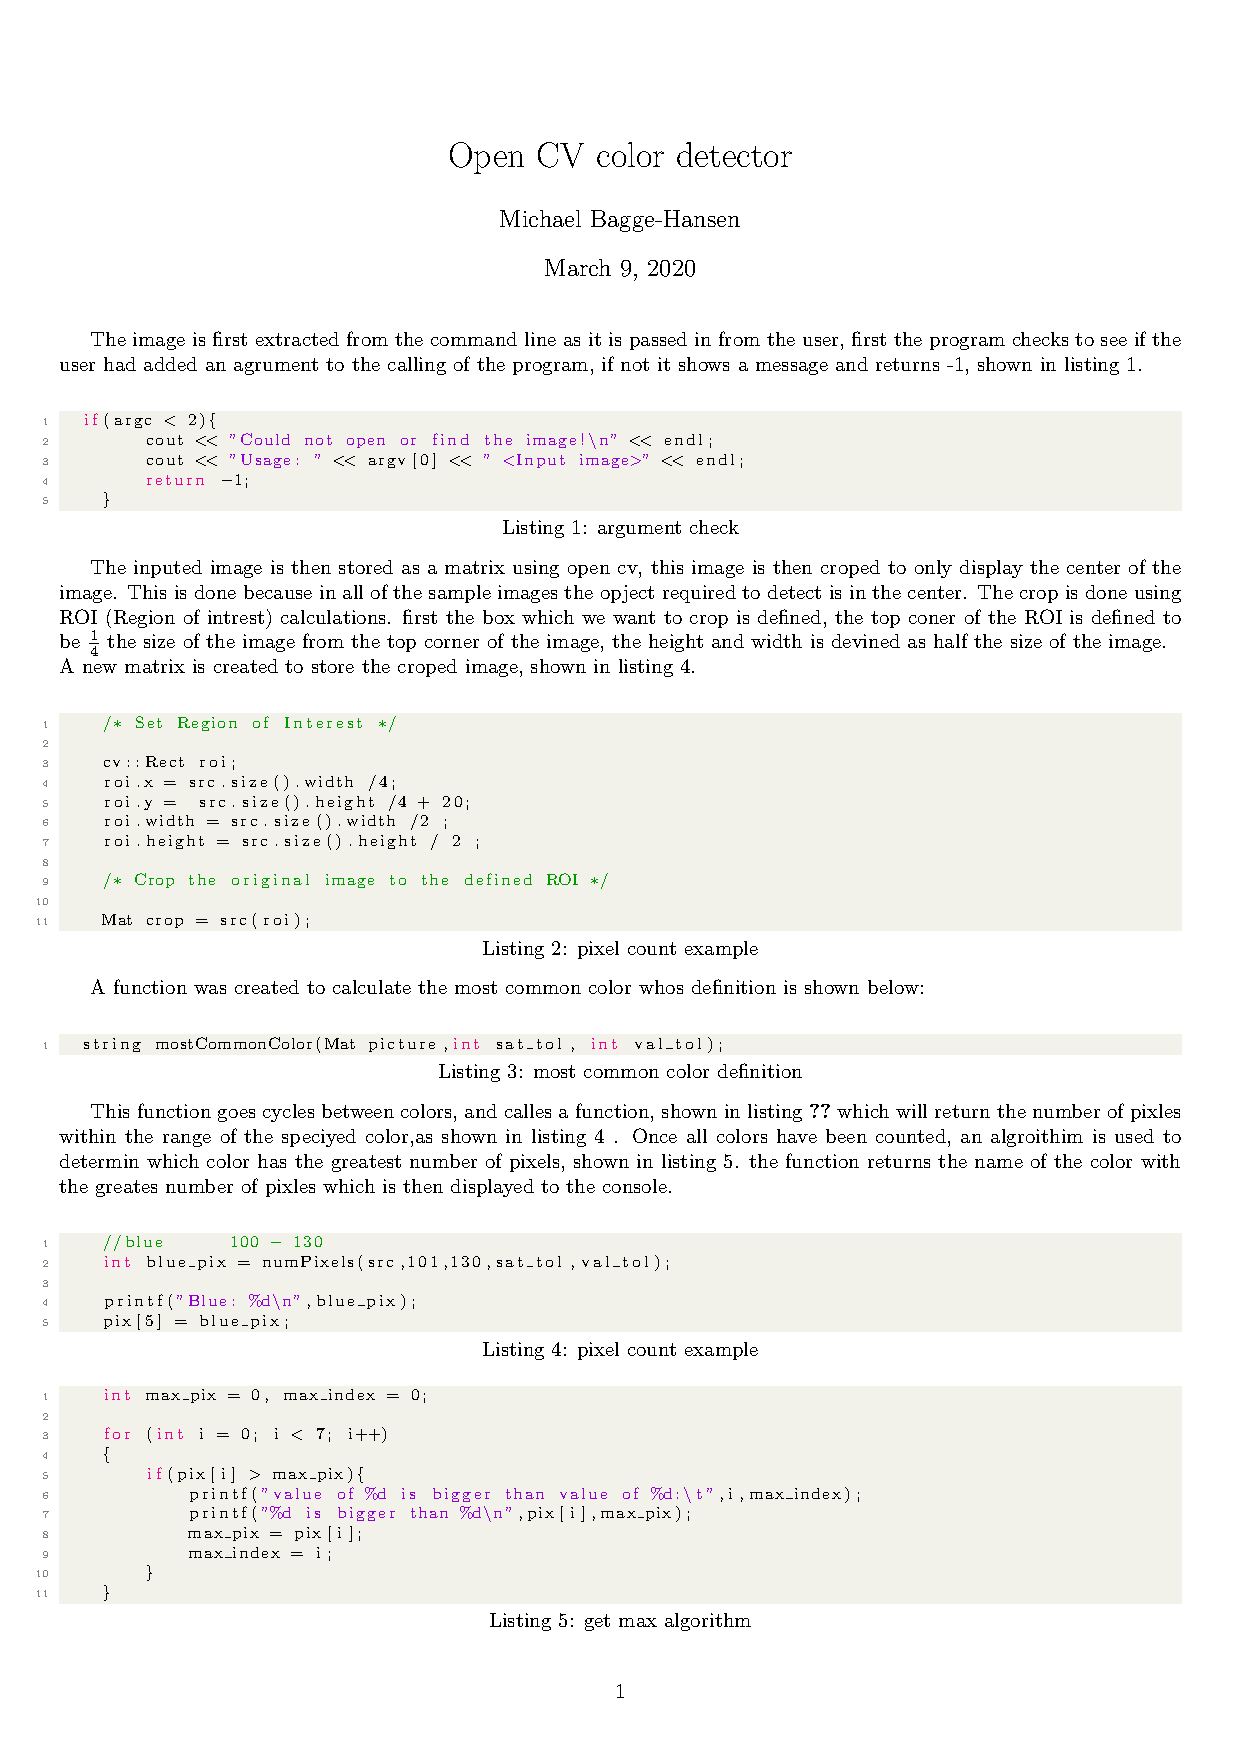
\includepdf[pages=-]{assets/code/open_cv_task.pdf}

	\section{Motor control arduino}
	\label{apx:arduino_motor_control}
\lstinputlisting[language=c,caption={Arduino motor code v1},label={lst:arduino_motor_v1}]{assets/code/arduino_motor_V1.0.txt}

\lstinputlisting[language=c,caption={Arduino motor code v1.1},label={lst:arduino_motor_v1.1}]{assets/code/arduino_motor_V1.1.txt}

\lstinputlisting[language=c,caption={Arduino motor code v2},label={lst:arduino_motor_v2}]{assets/code/arduino_motor_V2.txt}

	\section{Motor control Pi}
	\label{apx:pi_motor_control}

\lstinputlisting[language=c,caption={Pi motor code v1},label={lst:pi_motor_v1}]{assets/code/Motor_control_code_v1.cpp}

\lstinputlisting[language=c,caption={Pi motor code v2},label={lst:pi_motor_v2}]{assets/code/Motor_control_code_v2-0.cpp}

\lstinputlisting[language=c,caption={Pi motor code v2.1},label={lst:pi_motor_v2.1}]{assets/code/Motor_control_code_v2-1.cpp}

	\section{sensors}
	
\lstinputlisting[language=c,caption={arduino sensor code},label={lst:arduino_sensors}]{assets/code/arduino_sensors.txt}

\lstinputlisting[language=c,caption={Pi sensor code},label={lst:pi_sensors}]{assets/code/sensors.cpp}

	\section{Line following}
	
\lstinputlisting[language=c,caption={Line following V1},label={lst:line_following_v1}]{assets/code/line_follow_V1.cpp}

\lstinputlisting[language=c,caption={Line following V2},label={lst:line_following_v2}]{assets/code/line_follow_V2.cpp}

	\section{Symbol detect}

\lstinputlisting[language=c,caption={Symbol detect},label={lst:symbol_code}]{assets/code/symbol_detect.cpp}

	\section{Shape counter}

\lstinputlisting[language=c,caption={Shape counter},label={lst:shape_count}]{assets/code/shape_count.cpp}
	
	\section{Stop light detection}
	
\lstinputlisting[language=c,caption={Stop light detection},label={lst:stop_light}]{assets/code/stop_lights.cpp}

	
\bibliographystyle{ieeetr}	
\bibliography{ref}

\end{document}
